% This file was created with tikzplotlib v0.10.1.
\begin{figure}[t]
\centering

\definecolor{crimson2143940}{RGB}{214,39,40}
\definecolor{darkgray176}{RGB}{176,176,176}
\definecolor{darkorange25512714}{RGB}{255,127,14}
\definecolor{forestgreen4416044}{RGB}{44,160,44}
\definecolor{lightgray204}{RGB}{204,204,204}
\definecolor{mediumpurple148103189}{RGB}{148,103,189}
\definecolor{orchid227119194}{RGB}{227,119,194}
\definecolor{sienna1408675}{RGB}{140,86,75}
\definecolor{steelblue31119180}{RGB}{31,119,180}

%\resizebox{.9\linewidth}{!}{
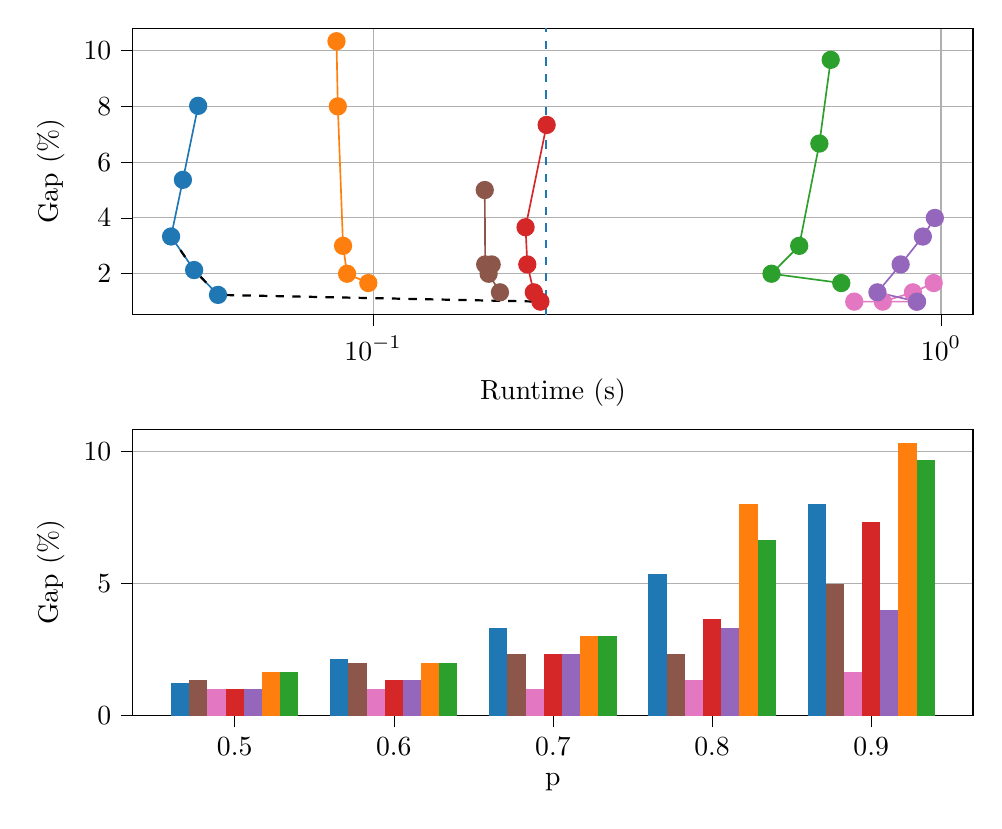
\begin{tikzpicture}



% --- top plot spanning full width ---
\begin{axis}[
at={(0,0)},
anchor=north west,
width=0.88\textwidth,
height=0.30\textwidth,
scale only axis,
log basis x={10},
tick align=outside,
tick pos=left,
%title={Pareto: Runtime vs Gap},
x grid style={darkgray176},
xlabel={Runtime (s)},
xmajorgrids,
xmin=0.0377572930471907, xmax=1.13855353365735,
xmode=log,
xtick style={color=black},
xtick={0.001,0.01,0.1,1,10,100},
xticklabels={
  \(\displaystyle 10^{-3}\),
  \(\displaystyle 10^{-2}\),
  \(\displaystyle 10^{-1}\),
  \(\displaystyle 10^{0}\),
  \(\displaystyle 10^{1}\),
  \(\displaystyle 10^{2}\)
},
y grid style={darkgray176},
ylabel={Gap (\%)},
ymajorgrids,
ymin=0.533333333333333, ymax=10.8,
ytick style={color=black},
]
% add your first plot data here
\addplot [semithick, steelblue31119180, mark=*, mark size=3, mark options={solid}]
table {%
0.0533245112893637 1.24148148148148
0.0484016584903002 2.13198653198653
0.0440802603455571 3.33414141414141
0.0462508742042507 5.36632996632997
0.0491994086856333 8.0179797979798
};
\addplot [semithick, sienna1408675, mark=*, mark size=3, mark options={solid}]
table {%
0.167278064165536 1.33333333333333
0.15974445293153 2
0.161742483200699 2.33333333333333
0.157533900999018 2.33333333333333
0.157259889768223 5
};
\addplot [semithick, orchid227119194, mark=*, mark size=3, mark options={solid}]
table {%
0.905844518799859 1
0.703446387465616 1
0.789790313632208 1
0.89236068273652 1.33333333333333
0.970661524065751 1.66666666666667
};
\addplot [semithick, crimson2143940, mark=*, mark size=3, mark options={solid}]
table {%
0.197063456933635 1
0.191888231933505 1.33333333333333
0.186879135599884 2.33333333333333
0.185584570733772 3.66666666666667
0.202103745898542 7.33333333333333
};
\addplot [semithick, mediumpurple148103189, mark=*, mark size=3, mark options={solid}]
table {%
0.907382919668453 1
0.772891245834277 1.33333333333333
0.84904408063303 2.33333333333333
0.928978601299847 3.33333333333333
0.975236967368498 4
};
\addplot [semithick, darkorange25512714, mark=*, mark size=3, mark options={solid}]
table {%
0.0980850083006468 1.66666666666667
0.08999063950032 2
0.0885351950991511 3
0.0866770093334101 8
0.086207477467057 10.3333333333333
};
\addplot [semithick, forestgreen4416044, mark=*, mark size=3, mark options={solid}]
table {%
0.66745852019861 1.66666666666667
0.502918167065945 2
0.56275247396843 3
0.610698752600001 6.66666666666667
0.63945260206771 9.66666666666667
};
\addplot [thick, black, dashed]
table {%
0.0440802603455571 3.33414141414141
0.0484016584903002 2.13198653198653
0.0533245112893637 1.24148148148148
0.197063456933635 1
};
\addplot [semithick, steelblue31119180, dashed]
table {%
0.201506736601663 0.533333333333335
0.201506736601663 10.8
};
\end{axis}



% --- bottom right plot ---
\begin{axis}[
%at={(0.46\textwidth,-0.42\textwidth)},
at={(0,-0.42\textwidth)},
anchor=north west,
width=0.88\textwidth,
height=0.30\textwidth,
%width=0.42\textwidth,
%height=0.28\textwidth,
scale only axis,
legend to name=sharedLegend,
legend columns=4,
legend cell align=left,
legend style={
  draw=lightgray204,
  /tikz/every even column/.append style={column sep=0.4cm}
},
tick align=outside,
tick pos=left,
%title={Gap Comparison},
x grid style={darkgray176},
xlabel={p},
xmin=-0.64, xmax=4.64,
xtick style={color=black},
xtick={0,1,2,3,4},
xticklabels={0.5,0.6,0.7,0.8,0.9},
y grid style={darkgray176},
ylabel={Gap (\%)},
ymajorgrids,
ymin=0, ymax=10.85,
ytick style={color=black},
]
% third plot data
\draw[draw=none,fill=steelblue31119180] (axis cs:-0.4,0) rectangle (axis cs:-0.285714285714286,1.24148148148148);
\addlegendimage{ybar,ybar legend,draw=none,fill=steelblue31119180}
\addlegendentry{GNN EGG}

\draw[draw=none,fill=steelblue31119180] (axis cs:0.6,0) rectangle (axis cs:0.714285714285714,2.13198653198653);
\draw[draw=none,fill=steelblue31119180] (axis cs:1.6,0) rectangle (axis cs:1.71428571428571,3.33414141414141);
\draw[draw=none,fill=steelblue31119180] (axis cs:2.6,0) rectangle (axis cs:2.71428571428571,5.36632996632997);
\draw[draw=none,fill=steelblue31119180] (axis cs:3.6,0) rectangle (axis cs:3.71428571428571,8.0179797979798);
\draw[draw=none,fill=sienna1408675] (axis cs:-0.285714285714286,0) rectangle (axis cs:-0.171428571428571,1.33333333333333);
\addlegendimage{ybar,ybar legend,draw=none,fill=sienna1408675}
\addlegendentry{MRF EGG}

\draw[draw=none,fill=sienna1408675] (axis cs:0.714285714285714,0) rectangle (axis cs:0.828571428571429,2);
\draw[draw=none,fill=sienna1408675] (axis cs:1.71428571428571,0) rectangle (axis cs:1.82857142857143,2.33333333333333);
\draw[draw=none,fill=sienna1408675] (axis cs:2.71428571428571,0) rectangle (axis cs:2.82857142857143,2.33333333333333);
\draw[draw=none,fill=sienna1408675] (axis cs:3.71428571428571,0) rectangle (axis cs:3.82857142857143,5);
\draw[draw=none,fill=orchid227119194] (axis cs:-0.171428571428571,0) rectangle (axis cs:-0.0571428571428571,1);
\addlegendimage{ybar,ybar legend,draw=none,fill=orchid227119194}
\addlegendentry{MRF GD}

\draw[draw=none,fill=orchid227119194] (axis cs:0.828571428571429,0) rectangle (axis cs:0.942857142857143,1);
\draw[draw=none,fill=orchid227119194] (axis cs:1.82857142857143,0) rectangle (axis cs:1.94285714285714,1);
\draw[draw=none,fill=orchid227119194] (axis cs:2.82857142857143,0) rectangle (axis cs:2.94285714285714,1.33333333333333);
\draw[draw=none,fill=orchid227119194] (axis cs:3.82857142857143,0) rectangle (axis cs:3.94285714285714,1.66666666666667);
\draw[draw=none,fill=crimson2143940] (axis cs:-0.0571428571428571,0) rectangle (axis cs:0.0571428571428571,1);
\addlegendimage{ybar,ybar legend,draw=none,fill=crimson2143940}
\addlegendentry{Pair MRF EGG}

\draw[draw=none,fill=crimson2143940] (axis cs:0.942857142857143,0) rectangle (axis cs:1.05714285714286,1.33333333333333);
\draw[draw=none,fill=crimson2143940] (axis cs:1.94285714285714,0) rectangle (axis cs:2.05714285714286,2.33333333333333);
\draw[draw=none,fill=crimson2143940] (axis cs:2.94285714285714,0) rectangle (axis cs:3.05714285714286,3.66666666666667);
\draw[draw=none,fill=crimson2143940] (axis cs:3.94285714285714,0) rectangle (axis cs:4.05714285714286,7.33333333333333);
\draw[draw=none,fill=mediumpurple148103189] (axis cs:0.0571428571428571,0) rectangle (axis cs:0.171428571428571,1);
\addlegendimage{ybar,ybar legend,draw=none,fill=mediumpurple148103189}
\addlegendentry{Pair MRF GD}

\draw[draw=none,fill=mediumpurple148103189] (axis cs:1.05714285714286,0) rectangle (axis cs:1.17142857142857,1.33333333333333);
\draw[draw=none,fill=mediumpurple148103189] (axis cs:2.05714285714286,0) rectangle (axis cs:2.17142857142857,2.33333333333333);
\draw[draw=none,fill=mediumpurple148103189] (axis cs:3.05714285714286,0) rectangle (axis cs:3.17142857142857,3.33333333333333);
\draw[draw=none,fill=mediumpurple148103189] (axis cs:4.05714285714286,0) rectangle (axis cs:4.17142857142857,4);
\draw[draw=none,fill=darkorange25512714] (axis cs:0.171428571428571,0) rectangle (axis cs:0.285714285714286,1.66666666666667);
\addlegendimage{ybar,ybar legend,draw=none,fill=darkorange25512714}
\addlegendentry{Tree MRF EGG}

\draw[draw=none,fill=darkorange25512714] (axis cs:1.17142857142857,0) rectangle (axis cs:1.28571428571429,2);
\draw[draw=none,fill=darkorange25512714] (axis cs:2.17142857142857,0) rectangle (axis cs:2.28571428571429,3);
\draw[draw=none,fill=darkorange25512714] (axis cs:3.17142857142857,0) rectangle (axis cs:3.28571428571429,8);
\draw[draw=none,fill=darkorange25512714] (axis cs:4.17142857142857,0) rectangle (axis cs:4.28571428571429,10.3333333333333);
\draw[draw=none,fill=forestgreen4416044] (axis cs:0.285714285714286,0) rectangle (axis cs:0.4,1.66666666666667);
\addlegendimage{ybar, ybar legend,draw=none,fill=forestgreen4416044}
\addlegendentry{Tree MRF GD}

\draw[draw=none,fill=forestgreen4416044] (axis cs:1.28571428571429,0) rectangle (axis cs:1.4,2);
\draw[draw=none,fill=forestgreen4416044] (axis cs:2.28571428571429,0) rectangle (axis cs:2.4,3);
\draw[draw=none,fill=forestgreen4416044] (axis cs:3.28571428571429,0) rectangle (axis cs:3.4,6.66666666666667);
\draw[draw=none,fill=forestgreen4416044] (axis cs:4.28571428571429,0) rectangle (axis cs:4.4,9.66666666666667);
\end{axis}



\end{tikzpicture}
\vspace{0.5em}
\makebox[\textwidth][c]{\pgfplotslegendfromname{sharedLegend}}
%}

\end{figure}